\subsection{Avaliação do CINTIL}
\label{subsec:resultados_cintil}
Nesta seção, demonstraremos os resultados obtidos com a transdução do CINTIL.

\subsubsection{Treinamento} 
\label{subsubsec:result_treino_cintil}

Na Tabela \ref{tab:resultados_treino_cintil}, podemos ver o relatório de cada treinamento do SP com cada \textit{fold} do CINTIL transduzido.
\begin{center}
    \begin{table}[h!]
    \centering
    % \begin{tabular}{c|c}
    %      &  \\
    %      & 
    % \end{tabular}
    \csvautotabular{tabelas/resultados_cintil_treino.csv}
    \caption{Resultados dos treinamentos do CINTIL, para os 10 \textit{folds}}
    \label{tab:resultados_treino_cintil}
\end{table}
\end{center}

Pode-se notar que, além do primeiro \textit{fold} (que abrange os últimos nove décimos do \textit{treeebank} para treinamento, e reserva o primeiro para testes), os resultados são bastante semelhantes. Deduz-se, então, que o primeiro décimo do \textit{dataset} temuma expressividade maior no processo de treino. O sexto \textit{fold} (reserva a 6ª parte para testes) parece ser o com melhores resultados gerais, como pode ser visto na Figura \ref{fig:treino_cintil}.
\begin{center}
    \begin{figure}[!ht]
    \centering
    % \includegraphics{}
    \includesvg[width=.8\textwidth]{imagens/treino_cintil}
    % \includesvg{imagens/cintil_pcfg}
    \caption[Gráfico de resultados do treinamento, usando o CINTIL transduzido]{Gráfico de resultados do treinamento do LexicalizedParser, usando o CINTIL transduzido}
    \label{fig:treino_cintil}
\end{figure}
\end{center}

As colunas necessitam de explicações próprias. O FAQ do SP é pouco informativo, e o do CoreNLP possui a mesma dificuldade.

Pelo código-fonte do SP\footnote{A referência foi a classe LexicalizedParser.java, que está disponível em \url{https://github.com/chbrown/stanford-parser/blob/master/edu/stanford/nlp/parser/lexparser/LexicalizedParser.java}}, \textit{States} representa a quantidade de Índices de Estado. Inferiu-se que é a quantidade de estados de transição da gramática gerada pelo treino. 

\textit{Tags}, por sua vez, representa a quantidade de Índices de \textit{Tags}. Seria a quantidade de \textit{Tags} registradas durante o treino (note que o número varia pouco).

\textit{Words}, de forma análoga, representa a quantidade de Índices de Palavras. Deduz-se que, a quantidade de palavras distintas verificadas pelo treinamento.

\textit{UnaryR} e \textit{BinaryR} correspondem, respectivamente, às quantidades de regras das gramáticas Unária e Binária. A descrição de suas classes é, na sequencia, 
\textquote{Mantém indexação eficiente das regras unárias da gramática}
\footnote{\textquote{\textit{Maintains efficient indexing of unary grammar rules}}}
e 
\textquote{Mantém indexação eficiente das regras binárias da gramática}
\footnote{\textquote{\textit{Maintains efficient indexing of binary grammar rules}}}
. Pelo Javadoc do SP\footnote{\url{https://nlp.stanford.edu/nlp/javadoc/javanlp/edu/stanford/nlp/parser/lexparser/package-summary.html}},
\begin{quote}
    \begin{itemize}
        \item \textit{Unary Grammar - consists of unary rewrite rules, one per line, each of which is of the form A -> B, followed by the normalized log probability.}
        \footnote{Gramática Unária - consiste em regras de reescrita unárias, uma por linha, cada qual na forma A -> B, seguida pela probabilidade log normalizada}
        \item \textit{Binary Grammar - consists of binary rewrite rules, one per line, each of which is of the form A -> B C, followed by the normalized log probability.}
        \footnote{Gramática Binária - consiste em regras de reescrita binárias, uma por linha, cada qual na forma A -> B C, seguida pela probabilidade log normalizada}
    \end{itemize}
\end{quote}

Cabe frisar que tal modelo, utilizando regras unárias e binárias, segue o padrão da Forma Normal de Chomsky.
% que pode ser visto em \cite[p~389]{Manning1999FoundationsNLP}.
Por \cite[p~389]{Manning1999FoundationsNLP}, Gramáticas na Forma Normal de Chomsky possuem apenas regras binárias e unárias, na forma:
\begin{center}
    \begin{equation}
\label{eq:forma_normal_chomsky}
    N^i \rightarrow N^j N^K
    
    N^i \rightarrow w^j
\end{equation}
\end{center}
Onde $N^i$ se refere à nós não-terminais (para este trabalho, nós internos das árvores e raiz), e $w^i$ se refere aos nós terminais (para este trabalho, nós contendo palavras).

Por fim, \textit{Taggings} se refere a \textquote{o número de regras (etiquetas reescritas como palavras) no \textit{Lexicon}}
\footnote{\textit{[\ldots]the number of rules (tag rewrites as word) in the Lexicon.} Tradução própria}.
\textit{Lexicon} é uma interface do software, descrita como
\begin{quote}
    \textquote{Uma interface entre \textit{lexicons} e o \textit{lexparser}. Sua responsabilidade primária é prover uma probabilidade condicional P(palavra|etiqueta), que é preenchida pelo método \textit{\#score}. Dentro do \textit{lexparser}, \textit{Strings} são representadas canonicamente, e etiquetas e palavras são geralmente representadas por inteiros}
    \footnote{\textquote{\textit{An interface for lexicons interfacing to lexparser. Its primary responsibility is to provide a conditional probability P(word|tag), which is fulfilled by the {\#score} method. Inside the lexparser, Strings are interned and tags and words are usually represented as integers.}} Tradução própria.}.
\end{quote}

\subsubsection{Avaliação} 
\label{subsubsec:result_aval_cintil}

Nos apêndices, a Tabela \ref{tab:cintil_result_full} traz os resultados completos dos testes com o CINTIL. Nesta seção serão utilizados um recorte dos dados.

Começando pelos dados da PCFG interna ao LexicalizedParser, podemos ver o seu resultado na Tabela \ref{tab:result_cintil_pcfg}, e na Figura \ref{fig:cintil_result_pcfg}.
\begin{center}
    \begin{table}[!h]
    \centering
    \begin{tabular}{|l|c|c|c|}
        \hline
        pcfg LP/LR & LP & LR & F1\\
        \hline
        fold 1 & 58.09 & 65.99 & 61.79\\
        fold 2 & 62.52 & 62.32 & 62.42\\
        fold 3 & 55.69 & 54.58 & 55.13\\
        fold 4 & 54.03 & 51.31 & 52.63\\
        fold 5 & 61.48 & 64.64 & 63.02\\
        fold 6 & 58.81 & 57.61 & 58.21\\
        fold 7 & 62.51 & 63.67 & 63.09\\
        fold 8 & 53.03 & 54.05 & 53.54\\
        fold 9 & 61.76 & 57.5 & 59.56\\
        fold 10 & 63.32 & 63.98 & 63.65\\
        \hline
    \end{tabular}
    % \csvautotabular{resultados-cintil-testes-pcfg.csv}
    \caption{Resultados do treinamento da PCFG do SP, usando dados do CINTIL}
    \label{tab:result_cintil_pcfg}
\end{table}
        % fold 1 & 45.43 & 45.04 & 45.24\\
        % fold 2 & 42.87 & 46.27 & 44.5\\
        % fold 3 & 39.8 & 42.86 & 41.27\\
        % fold 4 & 43.55 & 47.44 & 45.42\\
        % fold 5 & 41.82 & 43.7 & 42.74\\
        % fold 6 & 41.24 & 43.26 & 42.23\\
        % fold 7 & 44.51 & 45.43 & 44.97\\
        % fold 8 & 41.61 & 44.06 & 42.8\\
        % fold 9 & 38.85 & 44.39 & 41.43\\
        % fold 10 & 39.92 & 44.13 & 41.92\\
\end{center}

A média da \textit{F1-Score} é 59.304\%, e seu desvio padrão é de aprox. 4.208\%.

Fica claro que a simples transdução de árvores da língua portuguesa para os padrões da língua inglesa, conservando as palavras, é insuficiente para o bom resultado do \textit{parser}. Que se pese que as características que precisaram ser removidas, como pontuações, também tiveram elevada influencia nestes índices.

\begin{center}
    \begin{figure}[!ht]
    \centering
    % \includegraphics{}
    \includesvg[width=.8\textwidth]{imagens/cintil_pcfg}
    % \includesvg{imagens/cintil_pcfg}
    \caption[Gráfico de resultados dos testes usando o CINTIL transduzido]{Gráfico de resultados dos testes do PCFG do LexicalizedParser, usando o CINTIL transduzido}
    \label{fig:cintil_result_pcfg}
\end{figure}
\end{center}

\subsubsection{Análise de Erro dos treinamentos do SP com dados transduzidos do CINTIL}
\label{subsubsec:ec_cintil}

Foram separadas alguns exemplos de sentenças transduzidas, classificadas pelo \textit{Stanford Parser}. Serão exibidas as sentenças já em formato de árvore. Serão feitos comparativos entre as árvores das sentenças originais, em relação às árvores resultantes dos processo de transdução. Para incrementar o debate, também será demonstrada a árvore gerada pelo \textit{Stanford Parser} treinado com as gramáticas geradas por este trabalho. Para as análises a seguir, utilizou-se a gramática gerada a partir do sexto \textit{fold}. As imagens foram produzidas no \textit{website} jsSyntaxTree\footnote{\url{http://www.ironcreek.net/syntaxtree/}}.

\begin{center}
    \begin{figure}[!ht]
    \centering
    % \includegraphics{}
    \begin{minipage}{.45\textwidth}
        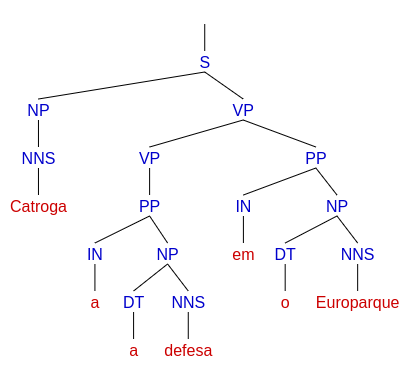
\includegraphics[width=\linewidth]{imagens/ec_cintil_sem_ponto_tree_trans.png}
        % \begin{forest}
        %     [
        %      [S 
        %       [NP 
        %       [NNS Catroga]
        %       ]
        %       [VP 
        %       [VP 
        %         [PP 
        %          [\textbf{IN a\_}]
        %          [NP 
        %           [\textbf{DT a}]
        %           [NNS defesa]
        %          ]
        %         ]
        %       ]
        %       [PP 
        %         [\textbf{IN em\_}]
        %         [NP 
        %          [\textbf{DT o}]
        %          [NNS Europarque]
        %         ]
        %       ]
        %       ]
        %      ]
        %     ]
        % \end{forest}
    \end{minipage}
    % 
    \begin{minipage}{.45\textwidth}
        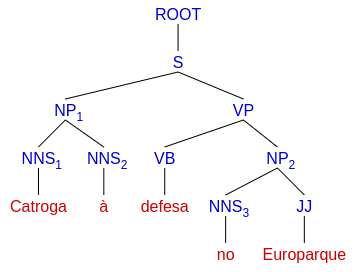
\includegraphics[width=\linewidth]{imagens/ec_cintil_sem_ponto_tree_sp.png}
        % \begin{forest}
        %     [ROOT
        %       [S
        %         [NP [NNS Catroga] [\textbf{JJ à}]]
        %         [VP [VB defesa]
        %           [NP [\textbf{NNS no}] [JJ Europarque]]]]]
        % \end{forest}
    \end{minipage}
    \caption[Estudo de caso CINTIL - Sentença transduzida sem pontuação]{Estudo da sentença eCTMP-000647/78121, \textquote{Catroga à defesa no Europarque}, que originalmente não possui nenhuma pontuação}
    \label{fig:ec_cintil_sem_ponto_tree}
\end{figure}
\end{center}

Na Figura \ref{fig:ec_cintil_sem_ponto_tree}, vemos o resultado da classificação de uma sentença originalmente sem pontuações. Se, por um lado, de fato a falta de pontuação ajudou no \textit{parsing}, as contrações de preposição (\textquote{à}, \textquote{no}) não são identificados. Neste momento, é importante lembrar que nenhuma modificação foi feita no Stanford Parser. Logo, não afetamos seu modelo de linguagem padrão, responsável por este tipo de tratamento

\begin{center}
    \begin{figure}[!ht]
    \centering
    a)
    \begin{minipage}{.45\textwidth}
        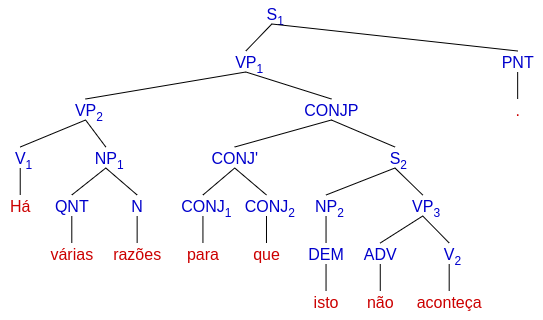
\includegraphics[width=\linewidth]{imagens/ec_cintil_conjp_tree_orig.png}
    \end{minipage}
    \hfill
    b)
    \begin{minipage}{.45\textwidth}
        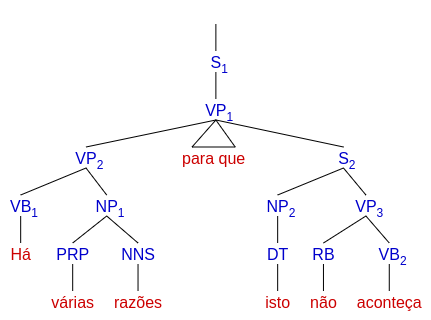
\includegraphics[width=\linewidth]{imagens/ec_cintil_conjp_tree_trans.png}
    \end{minipage}
    \hfill
    \vskip\floatsep
    c)
    \begin{minipage}{.45\textwidth}
        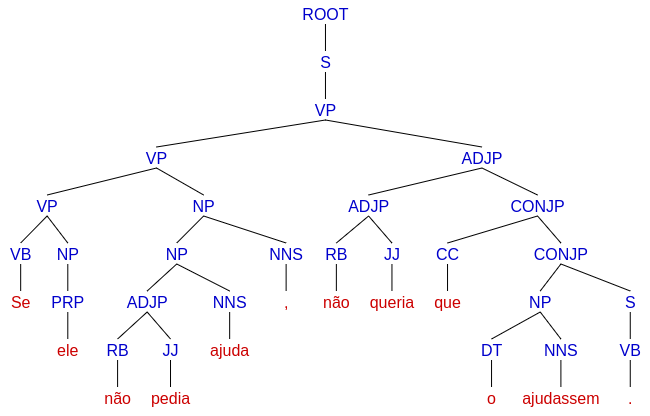
\includegraphics[width=\linewidth]{imagens/ec_cintil_conjp_tree_sp.png}
    \end{minipage}
    \caption[Estudo de caso CINTIL - Árvore da sentença transduzida com CONJP]{Estudo da sentença eCTMP-001150/117736, \textquote{Há várias razões para que isto não aconteça.}, que possui CONJP internamente. Em a), temos a árvore como se apresenta originalmente no CINTIL. Em b), temos a mesma sentença, pós transdução. Em c), temos o resultado da classificação do SP, utilizando a gramática gerada neste trabalho (após o processo de transdução)}
    \label{fig:ec_cintil_conjp_tree}
\end{figure}
\end{center}

Na Figura \ref{fig:ec_cintil_conjp_tree} podem ser vistas as problemáticas do tratamento de conjunções.

A confusão gerada pela falta de treinamento sobre pontuações permanece, sendo uma das maiores fontes de erros. O $VP_3$ \textquote{não aconteça} se torna um $ADJP$, considerando como núcleo o advérbio \textquote{não}. O esforço de manter a estrutura de conjunções, visto na Seção \ref{subsec:cintil-conj} é desfeito, convertendo o sintagma solto em \textit{flat structure} \textquote{para que} se converte num PP. Vale notar que ele não se torna um sintagma conjuntivo (CONJP), e \textquote{que} não é marcado como CC, que é a tendência tradicional do \textit{parser}. Também, apesar da tendência da língua inglesa, que costuma ter o núcleo do sintagma posicionado mais à direita \cite[p~40]{charniak97statistical}, isso não ocorre nem no PP, nem no ADJP.

\begin{center}
    \begin{figure}[!ht]
    \centering
    \begin{minipage}{.45\textwidth}
        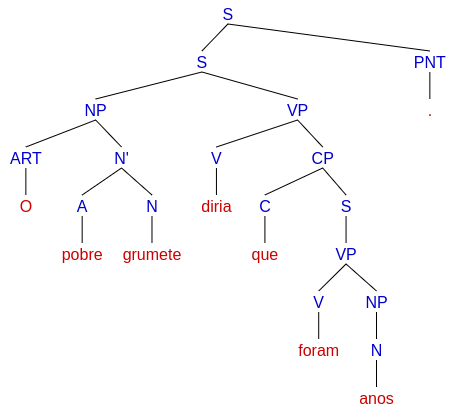
\includegraphics[width=\linewidth]{imagens/ec_cintil_cp_tree_orig.png}
        \caption{árvore original}
    \end{minipage}
    \hfill
    \begin{minipage}{.45\textwidth}
        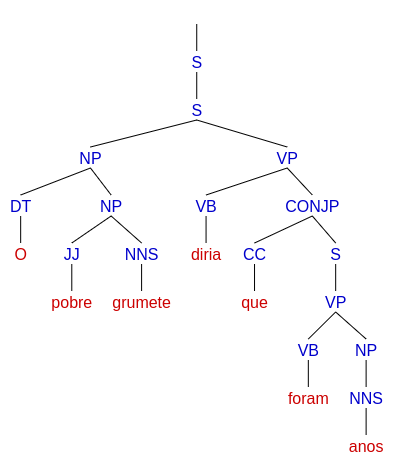
\includegraphics[width=\linewidth]{imagens/ec_cintil_cp_tree_trans.png}
        \caption{árvore transduzida}
    \end{minipage}
    \hfill
    \vskip\floatsep
    \begin{minipage}{.45\textwidth}
        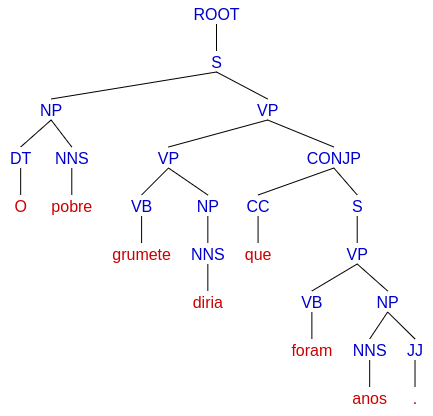
\includegraphics[width=\linewidth]{imagens/ec_cintil_cp_tree_sp.png}
        \caption{árvore gerada pelo SP}
    \end{minipage}
    \caption[Estudo de caso CINTIL - Árvore da sentença transduzida com CP]{Estudo da sentença eCTMP-000694/81773, \textquote{O pobre grumete diria que foram anos.}, que possui CP internamente.}
    \label{fig:ec_cintil_cp_tree}
\end{figure}
\end{center}

Na Figura \ref{fig:ec_cintil_cp_tree}, pode-se verificar as alterações realizadas sobre o sintagma CP, como visto na Seção \ref{subsec:cintil-c}. O sintagma em questão está acompanhando bem a estrutura da árvore original, e da árvore transduzida.

\begin{center}
    \begin{figure}[!ht]
    \centering
    \begin{minipage}{.45\textwidth}
        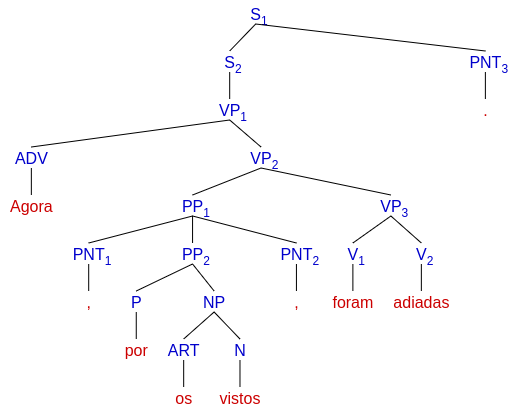
\includegraphics[width=\linewidth]{imagens/ec_cintil_virgula_tree_orig.png}
        \caption{árvore original}
    \end{minipage}
    \hfill
    \begin{minipage}{.45\textwidth}
        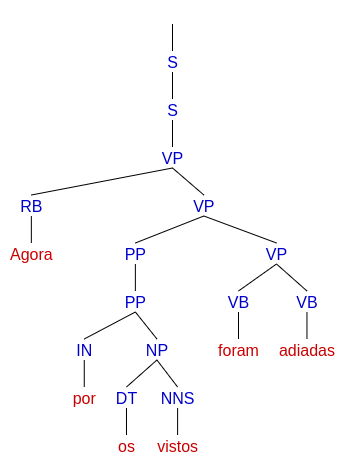
\includegraphics[width=\linewidth]{imagens/ec_cintil_virgula_tree_trans.png}
        \caption{árvore transduzida}
    \end{minipage}
    \hfill
    \vskip\floatsep
    \begin{minipage}{.45\textwidth}
        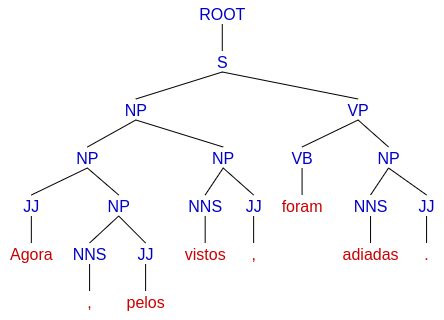
\includegraphics[width=\linewidth]{imagens/ec_cintil_virgula_tree_sp.png}
        \caption{árvore gerada pelo SP}
    \end{minipage}
    \caption[Estudo de caso CINTIL - Árvore da sentença transduzida com vírgulas]{Estudo da sentença eCTMP-001597/153293, \textquote{Agora, pelos vistos, foram adiadas.}, que possui vírgulas.}
    \label{fig:ec_cintil_virgula_tree}
\end{figure}
\end{center}

Por fim, a Figura \ref{fig:ec_cintil_virgula_tree} possui um exemplo utilizando vírgulas.
Pode-se notar a dificuldade léxica, onde palavras como \textquote{vistos} e \textquote{adiadas} são confundidos. Acredita-se que, se a contração da palavra \textquote{pelos} fosse detectada, a presença do Determinante resolveria tal problema. Os erros de marcação destes terminais afetam toda a marcação da árvore acima. Sem o treino utilizando pontuações, tais símbolos se tornam ou substantivos (NNS), ou adjetivos (JJ). Note-se também que, como demonstrado nas Figuras \ref{fig:ec_cintil_virgula_tree} e \ref{fig:ec_cintil_conjp_tree}, o mesmo sinal pode receber classificações diferentes em sentenças diferentes.